\documentclass[12pt]{article}

%packages
%\usepackage{latexsym}
\usepackage{graphicx}
\usepackage{color}
\usepackage{amsmath}
\usepackage{dsfont}
\usepackage{placeins}
\usepackage{amssymb}
\usepackage{wasysym}
\usepackage{abstract}
\usepackage{hyperref}
\usepackage{etoolbox}
\usepackage{datetime}
\usepackage{xcolor}
\usepackage{alphalph}
\settimeformat{ampmtime}

%\usepackage{pstricks,pst-node,pst-tree}

%\usepackage{algpseudocode}
%\usepackage{amsthm}
%\usepackage{hyperref}
%\usepackage{mathrsfs}
%\usepackage{amsfonts}
%\usepackage{bbding}
%\usepackage{listings}
%\usepackage{appendix}
\usepackage[margin=1in]{geometry}
%\geometry{papersize={8.5in,11in},total={6.5in,9in}}
%\usepackage{cancel}
%\usepackage{algorithmic, algorithm}

\makeatletter
\def\maxwidth{ %
  \ifdim\Gin@nat@width>\linewidth
    \linewidth
  \else
    \Gin@nat@width
  \fi
}
\makeatother

\definecolor{fgcolor}{rgb}{0.345, 0.345, 0.345}
\newcommand{\hlnum}[1]{\textcolor[rgb]{0.686,0.059,0.569}{#1}}%
\newcommand{\hlstr}[1]{\textcolor[rgb]{0.192,0.494,0.8}{#1}}%
\newcommand{\hlcom}[1]{\textcolor[rgb]{0.678,0.584,0.686}{\textit{#1}}}%
\newcommand{\hlopt}[1]{\textcolor[rgb]{0,0,0}{#1}}%
\newcommand{\hlstd}[1]{\textcolor[rgb]{0.345,0.345,0.345}{#1}}%
\newcommand{\hlkwa}[1]{\textcolor[rgb]{0.161,0.373,0.58}{\textbf{#1}}}%
\newcommand{\hlkwb}[1]{\textcolor[rgb]{0.69,0.353,0.396}{#1}}%
\newcommand{\hlkwc}[1]{\textcolor[rgb]{0.333,0.667,0.333}{#1}}%
\newcommand{\hlkwd}[1]{\textcolor[rgb]{0.737,0.353,0.396}{\textbf{#1}}}%

\usepackage{framed}
\makeatletter
\newenvironment{kframe}{%
 \def\at@end@of@kframe{}%
 \ifinner\ifhmode%
  \def\at@end@of@kframe{\end{minipage}}%
  \begin{minipage}{\columnwidth}%
 \fi\fi%
 \def\FrameCommand##1{\hskip\@totalleftmargin \hskip-\fboxsep
 \colorbox{shadecolor}{##1}\hskip-\fboxsep
     % There is no \\@totalrightmargin, so:
     \hskip-\linewidth \hskip-\@totalleftmargin \hskip\columnwidth}%
 \MakeFramed {\advance\hsize-\width
   \@totalleftmargin\z@ \linewidth\hsize
   \@setminipage}}%
 {\par\unskip\endMakeFramed%
 \at@end@of@kframe}
\makeatother

\definecolor{shadecolor}{rgb}{.77, .77, .77}
\definecolor{messagecolor}{rgb}{0, 0, 0}
\definecolor{warningcolor}{rgb}{1, 0, 1}
\definecolor{errorcolor}{rgb}{1, 0, 0}
\newenvironment{knitrout}{}{} % an empty environment to be redefined in TeX

\usepackage{alltt}
\usepackage[T1]{fontenc}

\newcommand{\qu}[1]{``#1''}
\newcounter{probnum}
\setcounter{probnum}{1}

%create definition to allow local margin changes
\def\changemargin#1#2{\list{}{\rightmargin#2\leftmargin#1}\item[]}
\let\endchangemargin=\endlist 

%allow equations to span multiple pages
\allowdisplaybreaks

%define colors and color typesetting conveniences
\definecolor{gray}{rgb}{0.5,0.5,0.5}
\definecolor{black}{rgb}{0,0,0}
\definecolor{white}{rgb}{1,1,1}
\definecolor{blue}{rgb}{0.5,0.5,1}
\newcommand{\inblue}[1]{\color{blue}#1 \color{black}}
\definecolor{green}{rgb}{0.133,0.545,0.133}
\newcommand{\ingreen}[1]{\color{green}#1 \color{black}}
\definecolor{yellow}{rgb}{1,1,0}
\newcommand{\inyellow}[1]{\color{yellow}#1 \color{black}}
\definecolor{orange}{rgb}{0.9,0.649,0}
\newcommand{\inorange}[1]{\color{orange}#1 \color{black}}
\definecolor{red}{rgb}{1,0.133,0.133}
\newcommand{\inred}[1]{\color{red}#1 \color{black}}
\definecolor{purple}{rgb}{0.58,0,0.827}
\newcommand{\inpurple}[1]{\color{purple}#1 \color{black}}
\definecolor{backgcode}{rgb}{0.97,0.97,0.8}
\definecolor{Brown}{cmyk}{0,0.81,1,0.60}
\definecolor{OliveGreen}{cmyk}{0.64,0,0.95,0.40}
\definecolor{CadetBlue}{cmyk}{0.62,0.57,0.23,0}

%define new math operators
\DeclareMathOperator*{\argmax}{arg\,max~}
\DeclareMathOperator*{\argmin}{arg\,min~}
\DeclareMathOperator*{\argsup}{arg\,sup~}
\DeclareMathOperator*{\arginf}{arg\,inf~}
\DeclareMathOperator*{\convolution}{\text{\Huge{$\ast$}}}
\newcommand{\infconv}[2]{\convolution^\infty_{#1 = 1} #2}
%true functions

%%%% GENERAL SHORTCUTS

%shortcuts for pure typesetting conveniences
\newcommand{\bv}[1]{\boldsymbol{#1}}

%shortcuts for compound constants
\newcommand{\BetaDistrConst}{\dfrac{\Gamma(\alpha + \beta)}{\Gamma(\alpha)\Gamma(\beta)}}
\newcommand{\NormDistrConst}{\dfrac{1}{\sqrt{2\pi\sigma^2}}}

%shortcuts for conventional symbols
\newcommand{\tsq}{\tau^2}
\newcommand{\tsqh}{\hat{\tau}^2}
\newcommand{\sigsq}{\sigma^2}
\newcommand{\sigsqsq}{\parens{\sigma^2}^2}
\newcommand{\sigsqovern}{\dfrac{\sigsq}{n}}
\newcommand{\tausq}{\tau^2}
\newcommand{\tausqalpha}{\tau^2_\alpha}
\newcommand{\tausqbeta}{\tau^2_\beta}
\newcommand{\tausqsigma}{\tau^2_\sigma}
\newcommand{\betasq}{\beta^2}
\newcommand{\sigsqvec}{\bv{\sigma}^2}
\newcommand{\sigsqhat}{\hat{\sigma}^2}
\newcommand{\sigsqhatmlebayes}{\sigsqhat_{\text{Bayes, MLE}}}
\newcommand{\sigsqhatmle}[1]{\sigsqhat_{#1, \text{MLE}}}
\newcommand{\bSigma}{\bv{\Sigma}}
\newcommand{\bSigmainv}{\bSigma^{-1}}
\newcommand{\thetavec}{\bv{\theta}}
\newcommand{\thetahat}{\hat{\theta}}
\newcommand{\thetahatmle}{\hat{\theta}_{\mathrm{MLE}}}
\newcommand{\thetavechatmle}{\hat{\thetavec}_{\mathrm{MLE}}}
\newcommand{\muhat}{\hat{\mu}}
\newcommand{\musq}{\mu^2}
\newcommand{\muvec}{\bv{\mu}}
\newcommand{\muhatmle}{\muhat_{\text{MLE}}}
\newcommand{\lambdahat}{\hat{\lambda}}
\newcommand{\lambdahatmle}{\lambdahat_{\text{MLE}}}
\newcommand{\etavec}{\bv{\eta}}
\newcommand{\alphavec}{\bv{\alpha}}
\newcommand{\minimaxdec}{\delta^*_{\mathrm{mm}}}
\newcommand{\ybar}{\bar{y}}
\newcommand{\xbar}{\bar{x}}
\newcommand{\Xbar}{\bar{X}}
\newcommand{\phat}{\hat{p}}
\newcommand{\Phat}{\hat{P}}
\newcommand{\Zbar}{\bar{Z}}
\newcommand{\iid}{~{\buildrel iid \over \sim}~}
\newcommand{\inddist}{~{\buildrel ind \over \sim}~}
\newcommand{\approxdist}{~{\buildrel approx \over \sim}~}
\newcommand{\equalsindist}{~{\buildrel d \over =}~}
\newcommand{\loglik}[1]{\ell\parens{#1}}
\newcommand{\thetahatkminone}{\thetahat^{(k-1)}}
\newcommand{\thetahatkplusone}{\thetahat^{(k+1)}}
\newcommand{\thetahatk}{\thetahat^{(k)}}
\newcommand{\half}{\frac{1}{2}}
\newcommand{\third}{\frac{1}{3}}
\newcommand{\twothirds}{\frac{2}{3}}
\newcommand{\fourth}{\frac{1}{4}}
\newcommand{\fifth}{\frac{1}{5}}
\newcommand{\sixth}{\frac{1}{6}}

%shortcuts for vector and matrix notation
\newcommand{\A}{\bv{A}}
\newcommand{\At}{\A^T}
\newcommand{\Ainv}{\inverse{\A}}
\newcommand{\B}{\bv{B}}
\newcommand{\K}{\bv{K}}
\newcommand{\Kt}{\K^T}
\newcommand{\Kinv}{\inverse{K}}
\newcommand{\Kinvt}{(\Kinv)^T}
\newcommand{\M}{\bv{M}}
\newcommand{\Bt}{\B^T}
\newcommand{\Q}{\bv{Q}}
\newcommand{\Qt}{\Q^T}
\newcommand{\R}{\bv{R}}
\newcommand{\Rt}{\R^T}
\newcommand{\Z}{\bv{Z}}
\newcommand{\X}{\bv{X}}
\newcommand{\Xsub}{\X_{\text{(sub)}}}
\newcommand{\Xsubadj}{\X_{\text{(sub,adj)}}}
\newcommand{\I}{\bv{I}}
\newcommand{\Y}{\bv{Y}}
\newcommand{\sigsqI}{\sigsq\I}
\renewcommand{\P}{\bv{P}}
\newcommand{\Psub}{\P_{\text{(sub)}}}
\newcommand{\Pt}{\P^T}
\newcommand{\Pii}{P_{ii}}
\newcommand{\Pij}{P_{ij}}
\newcommand{\IminP}{(\I-\P)}
\newcommand{\Xt}{\bv{X}^T}
\newcommand{\XtX}{\Xt\X}
\newcommand{\XtXinv}{\parens{\Xt\X}^{-1}}
\newcommand{\XtXinvXt}{\XtXinv\Xt}
\newcommand{\XXtXinvXt}{\X\XtXinvXt}
\newcommand{\x}{\bv{x}}
\newcommand{\onevec}{\bv{1}}
\newcommand{\oneton}{1, \ldots, n}
\newcommand{\yoneton}{y_1, \ldots, y_n}
\newcommand{\yonetonorder}{y_{(1)}, \ldots, y_{(n)}}
\newcommand{\Yoneton}{Y_1, \ldots, Y_n}
\newcommand{\iinoneton}{i \in \braces{\oneton}}
\newcommand{\onetom}{1, \ldots, m}
\newcommand{\jinonetom}{j \in \braces{\onetom}}
\newcommand{\xoneton}{x_1, \ldots, x_n}
\newcommand{\Xoneton}{X_1, \ldots, X_n}
\newcommand{\xt}{\x^T}
\newcommand{\y}{\bv{y}}
\newcommand{\yt}{\y^T}
\renewcommand{\c}{\bv{c}}
\newcommand{\ct}{\c^T}
\newcommand{\tstar}{\bv{t}^*}
\renewcommand{\u}{\bv{u}}
\renewcommand{\v}{\bv{v}}
\renewcommand{\a}{\bv{a}}
\newcommand{\s}{\bv{s}}
\newcommand{\yadj}{\y_{\text{(adj)}}}
\newcommand{\xjadj}{\x_{j\text{(adj)}}}
\newcommand{\xjadjM}{\x_{j \perp M}}
\newcommand{\yhat}{\hat{\y}}
\newcommand{\yhatsub}{\yhat_{\text{(sub)}}}
\newcommand{\yhatstar}{\yhat^*}
\newcommand{\yhatstarnew}{\yhatstar_{\text{new}}}
\newcommand{\z}{\bv{z}}
\newcommand{\zt}{\z^T}
\newcommand{\bb}{\bv{b}}
\newcommand{\bbt}{\bb^T}
\newcommand{\bbeta}{\bv{\beta}}
\newcommand{\beps}{\bv{\epsilon}}
\newcommand{\bepst}{\beps^T}
\newcommand{\e}{\bv{e}}
\newcommand{\Mofy}{\M(\y)}
\newcommand{\KofAlpha}{K(\alpha)}
\newcommand{\ellset}{\mathcal{L}}
\newcommand{\oneminalph}{1-\alpha}
\newcommand{\SSE}{\text{SSE}}
\newcommand{\SSEsub}{\text{SSE}_{\text{(sub)}}}
\newcommand{\MSE}{\text{MSE}}
\newcommand{\RMSE}{\text{RMSE}}
\newcommand{\SSR}{\text{SSR}}
\newcommand{\SST}{\text{SST}}
\newcommand{\JSest}{\delta_{\text{JS}}(\x)}
\newcommand{\Bayesest}{\delta_{\text{Bayes}}(\x)}
\newcommand{\EmpBayesest}{\delta_{\text{EmpBayes}}(\x)}
\newcommand{\BLUPest}{\delta_{\text{BLUP}}}
\newcommand{\MLEest}[1]{\hat{#1}_{\text{MLE}}}

%shortcuts for Linear Algebra stuff (i.e. vectors and matrices)
\newcommand{\twovec}[2]{\bracks{\begin{array}{c} #1 \\ #2 \end{array}}}
\newcommand{\threevec}[3]{\bracks{\begin{array}{c} #1 \\ #2 \\ #3 \end{array}}}
\newcommand{\fivevec}[5]{\bracks{\begin{array}{c} #1 \\ #2 \\ #3 \\ #4 \\ #5 \end{array}}}
\newcommand{\twobytwomat}[4]{\bracks{\begin{array}{cc} #1 & #2 \\ #3 & #4 \end{array}}}
\newcommand{\threebytwomat}[6]{\bracks{\begin{array}{cc} #1 & #2 \\ #3 & #4 \\ #5 & #6 \end{array}}}

%shortcuts for conventional compound symbols
\newcommand{\thetainthetas}{\theta \in \Theta}
\newcommand{\reals}{\mathbb{R}}
\newcommand{\complexes}{\mathbb{C}}
\newcommand{\rationals}{\mathbb{Q}}
\newcommand{\integers}{\mathbb{Z}}
\newcommand{\naturals}{\mathbb{N}}
\newcommand{\forallninN}{~~\forall n \in \naturals}
\newcommand{\forallxinN}[1]{~~\forall #1 \in \reals}
\newcommand{\matrixdims}[2]{\in \reals^{\,#1 \times #2}}
\newcommand{\inRn}[1]{\in \reals^{\,#1}}
\newcommand{\mathimplies}{\quad\Rightarrow\quad}
\newcommand{\mathlogicequiv}{\quad\Leftrightarrow\quad}
\newcommand{\eqncomment}[1]{\quad \text{(#1)}}
\newcommand{\limitn}{\lim_{n \rightarrow \infty}}
\newcommand{\limitN}{\lim_{N \rightarrow \infty}}
\newcommand{\limitd}{\lim_{d \rightarrow \infty}}
\newcommand{\limitt}{\lim_{t \rightarrow \infty}}
\newcommand{\limitsupn}{\limsup_{n \rightarrow \infty}~}
\newcommand{\limitinfn}{\liminf_{n \rightarrow \infty}~}
\newcommand{\limitk}{\lim_{k \rightarrow \infty}}
\newcommand{\limsupn}{\limsup_{n \rightarrow \infty}}
\newcommand{\limsupk}{\limsup_{k \rightarrow \infty}}
\newcommand{\floor}[1]{\left\lfloor #1 \right\rfloor}
\newcommand{\ceil}[1]{\left\lceil #1 \right\rceil}

%shortcuts for environments
\newcommand{\beqn}{\vspace{-0.25cm}\begin{eqnarray*}}
\newcommand{\eeqn}{\end{eqnarray*}}
\newcommand{\bneqn}{\vspace{-0.25cm}\begin{eqnarray}}
\newcommand{\eneqn}{\end{eqnarray}}

%shortcuts for mini environments
\newcommand{\parens}[1]{\left(#1\right)}
\newcommand{\squared}[1]{\parens{#1}^2}
\newcommand{\tothepow}[2]{\parens{#1}^{#2}}
\newcommand{\prob}[1]{\mathbb{P}\parens{#1}}
\newcommand{\cprob}[2]{\prob{#1~|~#2}}
\newcommand{\littleo}[1]{o\parens{#1}}
\newcommand{\bigo}[1]{O\parens{#1}}
\newcommand{\Lp}[1]{\mathbb{L}^{#1}}
\renewcommand{\arcsin}[1]{\text{arcsin}\parens{#1}}
\newcommand{\prodonen}[2]{\bracks{\prod_{#1=1}^n #2}}
\newcommand{\mysum}[4]{\sum_{#1=#2}^{#3} #4}
\newcommand{\sumonen}[2]{\sum_{#1=1}^n #2}
\newcommand{\infsum}[2]{\sum_{#1=1}^\infty #2}
\newcommand{\infprod}[2]{\prod_{#1=1}^\infty #2}
\newcommand{\infunion}[2]{\bigcup_{#1=1}^\infty #2}
\newcommand{\infinter}[2]{\bigcap_{#1=1}^\infty #2}
\newcommand{\infintegral}[2]{\int^\infty_{-\infty} #2 ~\text{d}#1}
\newcommand{\supthetas}[1]{\sup_{\thetainthetas}\braces{#1}}
\newcommand{\bracks}[1]{\left[#1\right]}
\newcommand{\braces}[1]{\left\{#1\right\}}
\newcommand{\set}[1]{\left\{#1\right\}}
\newcommand{\abss}[1]{\left|#1\right|}
\newcommand{\norm}[1]{\left|\left|#1\right|\right|}
\newcommand{\normsq}[1]{\norm{#1}^2}
\newcommand{\inverse}[1]{\parens{#1}^{-1}}
\newcommand{\rowof}[2]{\parens{#1}_{#2\cdot}}

%shortcuts for functionals
\newcommand{\realcomp}[1]{\text{Re}\bracks{#1}}
\newcommand{\imagcomp}[1]{\text{Im}\bracks{#1}}
\newcommand{\range}[1]{\text{range}\bracks{#1}}
\newcommand{\colsp}[1]{\text{colsp}\bracks{#1}}
\newcommand{\rowsp}[1]{\text{rowsp}\bracks{#1}}
\newcommand{\tr}[1]{\text{tr}\bracks{#1}}
\newcommand{\rank}[1]{\text{rank}\bracks{#1}}
\newcommand{\proj}[2]{\text{Proj}_{#1}\bracks{#2}}
\newcommand{\projcolspX}[1]{\text{Proj}_{\colsp{\X}}\bracks{#1}}
\newcommand{\median}[1]{\text{median}\bracks{#1}}
\newcommand{\mean}[1]{\text{mean}\bracks{#1}}
\newcommand{\dime}[1]{\text{dim}\bracks{#1}}
\renewcommand{\det}[1]{\text{det}\bracks{#1}}
\newcommand{\expe}[1]{\mathbb{E}\bracks{#1}}
\newcommand{\expeabs}[1]{\expe{\abss{#1}}}
\newcommand{\expesub}[2]{\mathbb{E}_{#1}\bracks{#2}}
\newcommand{\indic}[1]{\mathds{1}_{#1}}
\newcommand{\var}[1]{\mathbb{V}\text{ar}\bracks{#1}}
\newcommand{\cov}[2]{\mathbb{C}\text{ov}\bracks{#1, #2}}
\newcommand{\corr}[2]{\text{Corr}\bracks{#1, #2}}
\newcommand{\se}[1]{\mathbb{S}\text{E}\bracks{#1}}
\newcommand{\seest}[1]{\hat{\mathbb{S}\text{E}}\bracks{#1}}
\newcommand{\bias}[1]{\text{Bias}\bracks{#1}}
\newcommand{\derivop}[2]{\dfrac{\text{d}}{\text{d} #1}\bracks{#2}}
\newcommand{\partialop}[2]{\dfrac{\partial}{\partial #1}\bracks{#2}}
\newcommand{\secpartialop}[2]{\dfrac{\partial^2}{\partial #1^2}\bracks{#2}}
\newcommand{\mixpartialop}[3]{\dfrac{\partial^2}{\partial #1 \partial #2}\bracks{#3}}

%shortcuts for functions
\renewcommand{\exp}[1]{\mathrm{exp}\parens{#1}}
\renewcommand{\cos}[1]{\text{cos}\parens{#1}}
\renewcommand{\sin}[1]{\text{sin}\parens{#1}}
\newcommand{\sign}[1]{\text{sign}\parens{#1}}
\newcommand{\are}[1]{\mathrm{ARE}\parens{#1}}
\newcommand{\natlog}[1]{\ln\parens{#1}}
\newcommand{\oneover}[1]{\frac{1}{#1}}
\newcommand{\overtwo}[1]{\frac{#1}{2}}
\newcommand{\overn}[1]{\frac{#1}{n}}
\newcommand{\oneoversqrt}[1]{\oneover{\sqrt{#1}}}
\newcommand{\sqd}[1]{\parens{#1}^2}
\newcommand{\loss}[1]{\ell\parens{\theta, #1}}
\newcommand{\losstwo}[2]{\ell\parens{#1, #2}}
\newcommand{\cf}{\phi(t)}

%English language specific shortcuts
\newcommand{\ie}{\textit{i.e.} }
\newcommand{\AKA}{\textit{AKA} }
\renewcommand{\iff}{\textit{iff}}
\newcommand{\eg}{\textit{e.g.} }
\newcommand{\st}{\textit{s.t.} }
\newcommand{\wrt}{\textit{w.r.t.} }
\newcommand{\mathst}{~~\text{\st}~~}
\newcommand{\mathand}{~~\text{and}~~}
\newcommand{\ala}{\textit{a la} }
\newcommand{\ppp}{posterior predictive p-value}
\newcommand{\dd}{dataset-to-dataset}

%shortcuts for distribution titles
\newcommand{\logistic}[2]{\mathrm{Logistic}\parens{#1,\,#2}}
\newcommand{\bernoulli}[1]{\mathrm{Bernoulli}\parens{#1}}
\newcommand{\betanot}[2]{\mathrm{Beta}\parens{#1,\,#2}}
\newcommand{\stdbetanot}{\betanot{\alpha}{\beta}}
\newcommand{\multnormnot}[3]{\mathcal{N}_{#1}\parens{#2,\,#3}}
\newcommand{\normnot}[2]{\mathcal{N}\parens{#1,\,#2}}
\newcommand{\classicnormnot}{\normnot{\mu}{\sigsq}}
\newcommand{\stdnormnot}{\normnot{0}{1}}
\newcommand{\uniformdiscrete}[1]{\mathrm{Uniform}\parens{\braces{#1}}}
\newcommand{\uniform}[2]{\mathrm{U}\parens{#1,\,#2}}
\newcommand{\stduniform}{\uniform{0}{1}}
\newcommand{\geometric}[1]{\mathrm{Geometric}\parens{#1}}
\newcommand{\hypergeometric}[3]{\mathrm{Hypergeometric}\parens{#1,\,#2,\,#3}}
\newcommand{\exponential}[1]{\mathrm{Exp}\parens{#1}}
\newcommand{\gammadist}[2]{\mathrm{Gamma}\parens{#1, #2}}
\newcommand{\poisson}[1]{\mathrm{Poisson}\parens{#1}}
\newcommand{\binomial}[2]{\mathrm{Binomial}\parens{#1,\,#2}}
\newcommand{\negbin}[2]{\mathrm{NegBin}\parens{#1,\,#2}}
\newcommand{\rayleigh}[1]{\mathrm{Rayleigh}\parens{#1}}
\newcommand{\multinomial}[2]{\mathrm{Multinomial}\parens{#1,\,#2}}
\newcommand{\gammanot}[2]{\mathrm{Gamma}\parens{#1,\,#2}}
\newcommand{\cauchynot}[2]{\text{Cauchy}\parens{#1,\,#2}}
\newcommand{\invchisqnot}[1]{\text{Inv}\chisq{#1}}
\newcommand{\invscaledchisqnot}[2]{\text{ScaledInv}\ncchisq{#1}{#2}}
\newcommand{\invgammanot}[2]{\text{InvGamma}\parens{#1,\,#2}}
\newcommand{\chisq}[1]{\chi^2_{#1}}
\newcommand{\ncchisq}[2]{\chi^2_{#1}\parens{#2}}
\newcommand{\ncF}[3]{F_{#1,#2}\parens{#3}}

%shortcuts for PDF's of common distributions
\newcommand{\logisticpdf}[3]{\oneover{#3}\dfrac{\exp{-\dfrac{#1 - #2}{#3}}}{\parens{1+\exp{-\dfrac{#1 - #2}{#3}}}^2}}
\newcommand{\betapdf}[3]{\dfrac{\Gamma(#2 + #3)}{\Gamma(#2)\Gamma(#3)}#1^{#2-1} (1-#1)^{#3-1}}
\newcommand{\normpdf}[3]{\frac{1}{\sqrt{2\pi#3}}\exp{-\frac{1}{2#3}(#1 - #2)^2}}
\newcommand{\normpdfvarone}[2]{\dfrac{1}{\sqrt{2\pi}}e^{-\half(#1 - #2)^2}}
\newcommand{\chisqpdf}[2]{\dfrac{1}{2^{#2/2}\Gamma(#2/2)}\; {#1}^{#2/2-1} e^{-#1/2}}
\newcommand{\invchisqpdf}[2]{\dfrac{2^{-\overtwo{#1}}}{\Gamma(#2/2)}\,{#1}^{-\overtwo{#2}-1}  e^{-\oneover{2 #1}}}
\newcommand{\exponentialpdf}[2]{#2\exp{-#2#1}}
\newcommand{\poissonpdf}[2]{\dfrac{e^{-#1} #1^{#2}}{#2!}}
\newcommand{\binomialpdf}[3]{\binom{#2}{#1}#3^{#1}(1-#3)^{#2-#1}}
\newcommand{\rayleighpdf}[2]{\dfrac{#1}{#2^2}\exp{-\dfrac{#1^2}{2 #2^2}}}
\newcommand{\gammapdf}[3]{\dfrac{#3^#2}{\Gamma\parens{#2}}#1^{#2-1}\exp{-#3 #1}}
\newcommand{\cauchypdf}[3]{\oneover{\pi} \dfrac{#3}{\parens{#1-#2}^2 + #3^2}}
\newcommand{\Gammaf}[1]{\Gamma\parens{#1}}

%shortcuts for miscellaneous typesetting conveniences
\newcommand{\notesref}[1]{\marginpar{\color{gray}\tt #1\color{black}}}

%%%% DOMAIN-SPECIFIC SHORTCUTS

%Real analysis related shortcuts
\newcommand{\zeroonecl}{\bracks{0,1}}
\newcommand{\forallepsgrzero}{\forall \epsilon > 0~~}
\newcommand{\lessthaneps}{< \epsilon}
\newcommand{\fraccomp}[1]{\text{frac}\bracks{#1}}

%Bayesian related shortcuts
\newcommand{\yrep}{y^{\text{rep}}}
\newcommand{\yrepisq}{(\yrep_i)^2}
\newcommand{\yrepvec}{\bv{y}^{\text{rep}}}


%Probability shortcuts
\newcommand{\SigField}{\mathcal{F}}
\newcommand{\ProbMap}{\mathcal{P}}
\newcommand{\probtrinity}{\parens{\Omega, \SigField, \ProbMap}}
\newcommand{\convp}{~{\buildrel p \over \rightarrow}~}
\newcommand{\convLp}[1]{~{\buildrel \Lp{#1} \over \rightarrow}~}
\newcommand{\nconvp}{~{\buildrel p \over \nrightarrow}~}
\newcommand{\convae}{~{\buildrel a.e. \over \longrightarrow}~}
\newcommand{\convau}{~{\buildrel a.u. \over \longrightarrow}~}
\newcommand{\nconvau}{~{\buildrel a.u. \over \nrightarrow}~}
\newcommand{\nconvae}{~{\buildrel a.e. \over \nrightarrow}~}
\newcommand{\convd}{~{\buildrel \mathcal{D} \over \rightarrow}~}
\newcommand{\nconvd}{~{\buildrel \mathcal{D} \over \nrightarrow}~}
\newcommand{\withprob}{~~\text{w.p.}~~}
\newcommand{\io}{~~\text{i.o.}}

\newcommand{\Acl}{\bar{A}}
\newcommand{\ENcl}{\bar{E}_N}
\newcommand{\diam}[1]{\text{diam}\parens{#1}}

\newcommand{\taua}{\tau_a}

\newcommand{\myint}[4]{\int_{#2}^{#3} #4 \,\text{d}#1}
\newcommand{\laplacet}[1]{\mathscr{L}\bracks{#1}}
\newcommand{\laplaceinvt}[1]{\mathscr{L}^{-1}\bracks{#1}}
\renewcommand{\min}[1]{\text{min}\braces{#1}}
\renewcommand{\max}[1]{\text{max}\braces{#1}}

\newcommand{\Vbar}[1]{\bar{V}\parens{#1}}
\newcommand{\expnegrtau}{\exp{-r\tau}}

%%% problem typesetting
\definecolor{darkgrey}{rgb}{0.10,0.10,0.9}

\newcommand{\problem}[1]{\noindent \colorbox{black}{{\color{yellow} \large{\textsf{\textbf{Problem \arabic{probnum}}}}~}} \addtocounter{probnum}{1} \vspace{0.2cm} \\ \iftoggle{professormode}{}{\color{darkgrey}} #1}

\newcommand{\easysubproblem}[1]{\ingreen{\item} \iftoggle{professormode}{}{\color{darkgrey}} [easy] #1 \color{black} }
\newcommand{\intermediatesubproblem}[1]{\inorange{\item} \iftoggle{professormode}{}{\color{darkgrey}} [harder] #1 \color{black} }
\newcommand{\hardsubproblem}[1]{\inred{\item} \iftoggle{professormode}{}{\color{darkgrey}} [difficult] #1 \color{black} }
\newcommand{\extracreditsubproblem}[1]{\inpurple{\item} \iftoggle{professormode}{}{\color{darkgrey}} [E.C.] #1 \color{black} }


\newcommand{\spc}[1]{\iftoggle{professormode}{\\ \vspace{#1cm}}{\\ \vspace{-0.3cm}}}

\makeatletter
\newalphalph{\alphmult}[mult]{\@alph}{26}
\renewcommand{\labelenumi}{(\alphmult{\value{enumi}})}

\newcommand{\support}[1]{\text{Supp}\bracks{#1}}
\newcommand{\mode}[1]{\text{Mode}\bracks{#1}}
\newcommand{\IQR}[1]{\text{IQR}\bracks{#1}}
\newcommand{\quantile}[2]{\text{Quantile}\bracks{#1,\,#2}}


\newcommand{\thetahatmap}{\hat{\theta}_{\mathrm{MAP}}}
\newcommand{\thetahatmae}{\hat{\theta}_{\mathrm{MMAE}}}
\newcommand{\thetahatmmse}{\hat{\theta}_{\mathrm{MMSE}}}
\usepackage{multicol}

\title{Math 390 / 650 Spring \the\year \\ Final Examination}
\author{Professor Adam Kapelner}

\date{Monday, May 23}

\begin{document}
\maketitle

\noindent Full Name \line(1,0){410}

\thispagestyle{empty}

\section*{Code of Academic Integrity}

\footnotesize
Since the college is an academic community, its fundamental purpose is the pursuit of knowledge. Essential to the success of this educational mission is a commitment to the principles of academic integrity. Every member of the college community is responsible for upholding the highest standards of honesty at all times. Students, as members of the community, are also responsible for adhering to the principles and spirit of the following Code of Academic Integrity.

Activities that have the effect or intention of interfering with education, pursuit of knowledge, or fair evaluation of a student's performance are prohibited. Examples of such activities include but are not limited to the following definitions:

\paragraph{Cheating} Using or attempting to use unauthorized assistance, material, or study aids in examinations or other academic work or preventing, or attempting to prevent, another from using authorized assistance, material, or study aids. Example: using an unauthorized cheat sheet in a quiz or exam, altering a graded exam and resubmitting it for a better grade, etc.
\\

\noindent I acknowledge and agree to uphold this Code of Academic Integrity. \\

\begin{center}
\line(1,0){250} ~~~ \line(1,0){100}\\
~~~~~~~~~~~~~~~~~~~~~signature~~~~~~~~~~~~~~~~~~~~~~~~~~~~~~~~~~~~~~~~~~~~~ date
\end{center}

\normalsize

\section*{Instructions}

This exam is seventy five minutes and closed-book. You are allowed \textbf{three} pages (front and back) of a \qu{cheat sheet.} You may use a graphing calculator of your choice. Please read the questions carefully. If the question reads \qu{compute,} this means the solution will be a number otherwise you can leave the answer in \textit{any} widely accepted mathematical notation which could be resolved to an exact or approximate number with the use of a computer. I advise you to skip problems marked \qu{[Extra Credit]} until you have finished the other questions on the exam, then loop back. I also advise you to use pencil. The exam is 100 points total plus extra credit. Partial credit will be granted for incomplete answers on most of the questions. \fbox{Box} in your final answers. NO FOOD but drinks okay. Good luck!

\pagebreak

\problem You take a sample of $n=200$ American people at random and measure their heights. According to \href{https://www.usablestats.com/lessons/normal}{this approximation}, male height is normally distributed with mean $\theta_M = 70$ inches and $\sigsq_M = 4^2$ squared-inches and female height is normally distributed with mean $\theta_F = 65$ inches and $\sigsq_F = 3.5^2$ squared-inches. 

\begin{figure}[h]
\centering
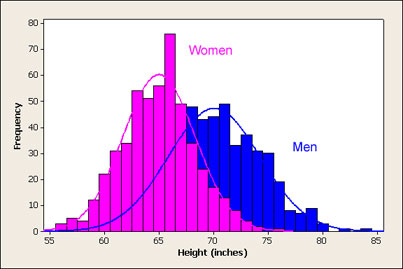
\includegraphics[width=4in]{men_women_height_histogram.jpg}
\end{figure}

\noindent We can assume this approximation is the truth i.e. $\theta_M, \theta_F, \sigsq_M, \sigsq_F$ are known and male heights are $\iid \normnot{\theta_M}{\sigsq_M}$ and female heights are $\iid \normnot{\theta_F}{\sigsq_F}$. We don't know the \emph{proportion} of males in our sample of $n$ people and we'll denote this proportion $\rho$ which is our main target of inference with $\support{\rho} = \zeroonecl$. Let $X_1, X_2, \ldots, X_n$ denote the measured heights in the sample.


\benum

\subquestionwithpoints{3} Write out the explicit PDF of the likelihood of the data given all the parameters: $\theta_M, \theta_F, \sigsq_M, \sigsq_F, \rho$.\spc{4}

\subquestionwithpoints{3} Why would it be difficult to find a closed-form solution for $\doublehat{\rho}_{\text{MLE}}$ given the likelihood you found in (a)? Write a couple sentences in English to answer.\spc{4}

We now \qu{augment the data} by introducing the parameters $I_1, I_2, \ldots, I_n$

\beqn
I_i := \begin{cases}
	1 ~~~ \text{if the $i$th data point is male, coming from the}~\normnot{\theta_M}{\sigsq_M} \text{distribution}\\
	 0 ~~~\text{if the $i$th data point is female, coming from the}~\normnot{\theta_F}{\sigsq_F} \text{distribution}
\end{cases}
\eeqn
\subquestionwithpoints{4} Write out the explicit PDF of the likelihood of the data given all the parameters and the parameters under data augmentation $\theta_M, \theta_F, \sigsq_M, \sigsq_F, \rho, I_1, I_2, \ldots, I_n$. Simplify as much as possible.\spc{5}


\subquestionwithpoints{3} Since $\theta_M, \theta_F, \sigsq_M, \sigsq_F$ are assumed known constants, we do not need to specify a prior for them. Specify the Laplace prior for $\rho$ explicitly. Do not simply write $\prob{\rho} \propto 1$. You need to write $\prob{\rho} = $ a legal distribution.\spc{0.3}

\subquestionwithpoints{3} Specify the Laplace prior for all the $I_i$'s explicitly. Do not simply write $\prob{I_i} \propto 1$. You need to write $\forall i~~\prob{I_i} = $ a legal distribution.\spc{0.3}

\subquestionwithpoints{4} Regardless of what you wrote for the previous two questions, you can now assume that $\prob{\rho, I_1, I_2, \ldots, I_n} \propto 1$. Find the kernel of the posterior as best as possible $k(\rho, I_1, I_2, \ldots, I_n\,|\,X_1, X_2, \ldots, X_n, \theta_M, \theta_F, \sigsq_M, \sigsq_F)$.\spc{6}

\subquestionwithpoints{4} The kernel you found in the previous example is not any known distribution that you know how to sample from. Thus we will employ a Gibbs sampler. Find the conditional distribution $\cprob{\rho}{I_1, I_2, \ldots, I_n, \theta_M, \theta_F, \sigsq_M, \sigsq_F, X_1, X_2, \ldots, X_n}$. It will be a known distribution. Compute its parameters.\spc{5.2}


\begin{figure}[h]
\centering
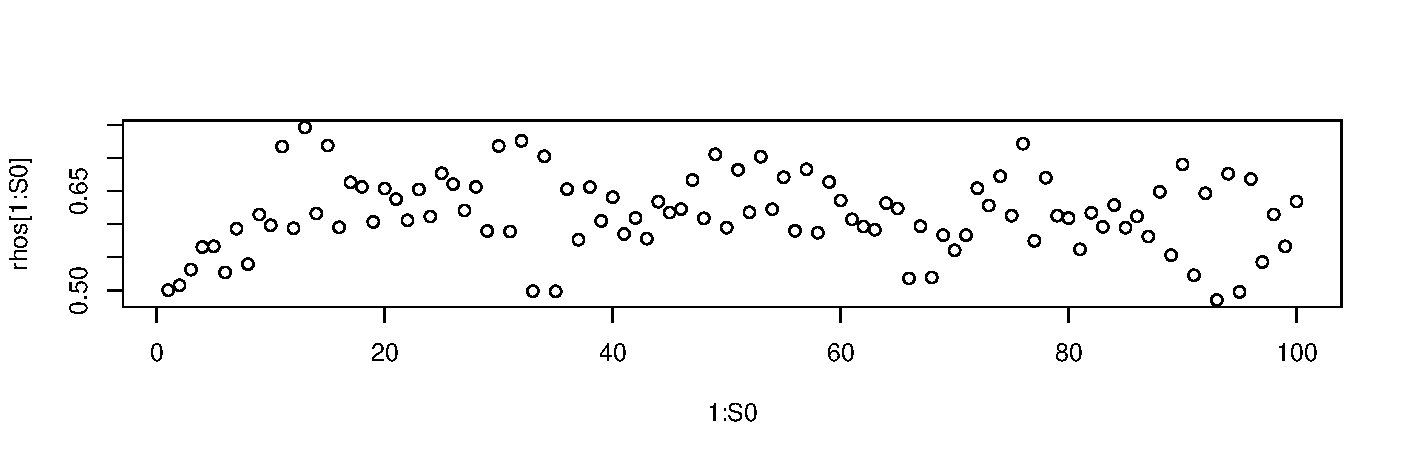
\includegraphics[width=5in]{burn}
\end{figure}
\vspace{-0.5cm}
\subquestionwithpoints{1} Above is the first 100 samples from the Gibbs sampler's conditional distribution $\cprob{\rho}{I_1, I_2, \ldots, I_n, \theta_M, \theta_F, \sigsq_M, \sigsq_F, X_1, X_2, \ldots, X_n}$. At what approximate iteration number would you burn?\spc{0}

\begin{figure}[h]
\centering
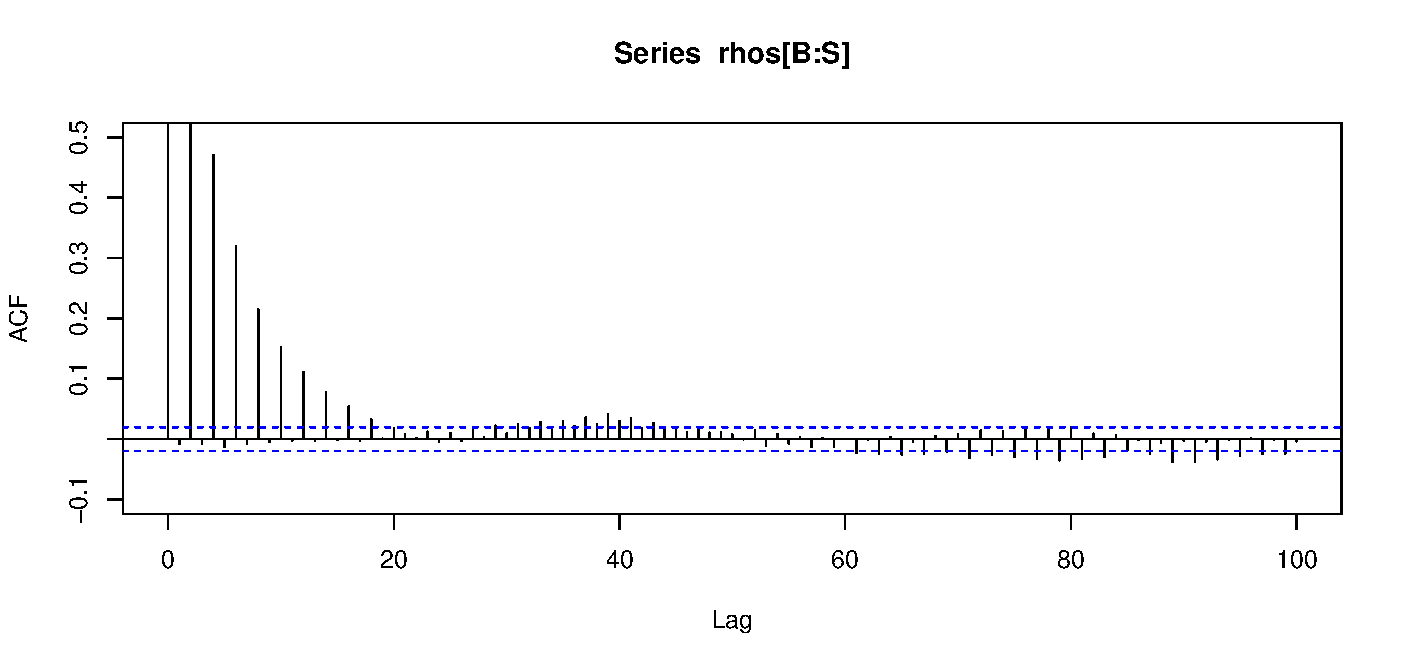
\includegraphics[width=5in]{ar}
\end{figure}
\vspace{-0.5cm}
\subquestionwithpoints{2} Above is an autocorrelation plot of post-burned samples from the Gibbs sampler's conditional distribution  $\cprob{\rho}{I_1, I_2, \ldots, I_n, \theta_M, \theta_F, \sigsq_M, \sigsq_F, X_1, X_2, \ldots, X_n}$. At what approximate iteration number would you thin?\spc{0}

\begin{figure}[h]
\centering
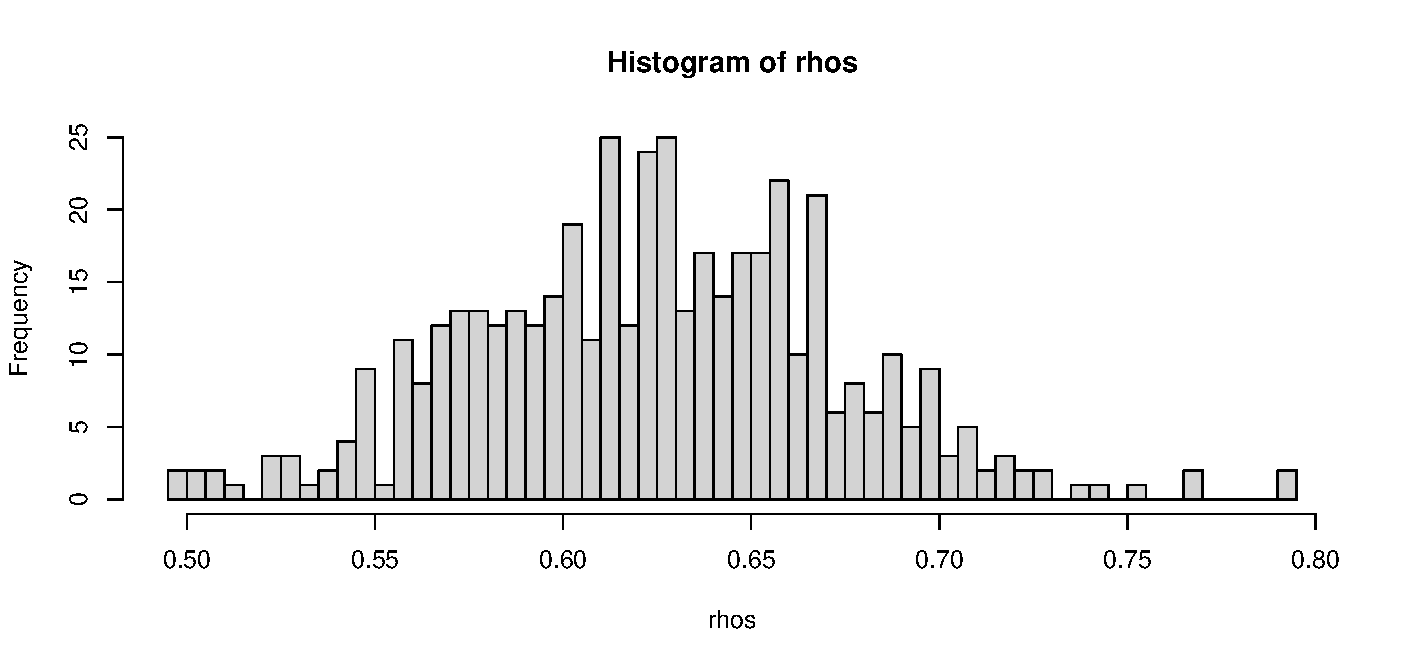
\includegraphics[width=5in]{rhos}
\end{figure}
\vspace{-0.5cm}
\subquestionwithpoints{2} Above is the post-burned and thinned samples from the Gibbs sampler's conditional distribution  $\cprob{\rho}{I_1, I_2, \ldots, I_n, \theta_M, \theta_F, \sigsq_M, \sigsq_F, X_1, X_2, \ldots, X_n}$. Estimate $\doublehat{\rho}_{\text{MMAE}}$.\spc{0}

\subquestionwithpoints{2} Provide an estimated $CR_{\rho, 95\%}$.\spc{0}

\subquestionwithpoints{5} Test the theory that this sample has an equal number of men and women. Show all work and be explicit about your assumptions. Write a concluding statement.\spc{4}

\begin{figure}[h]
\centering
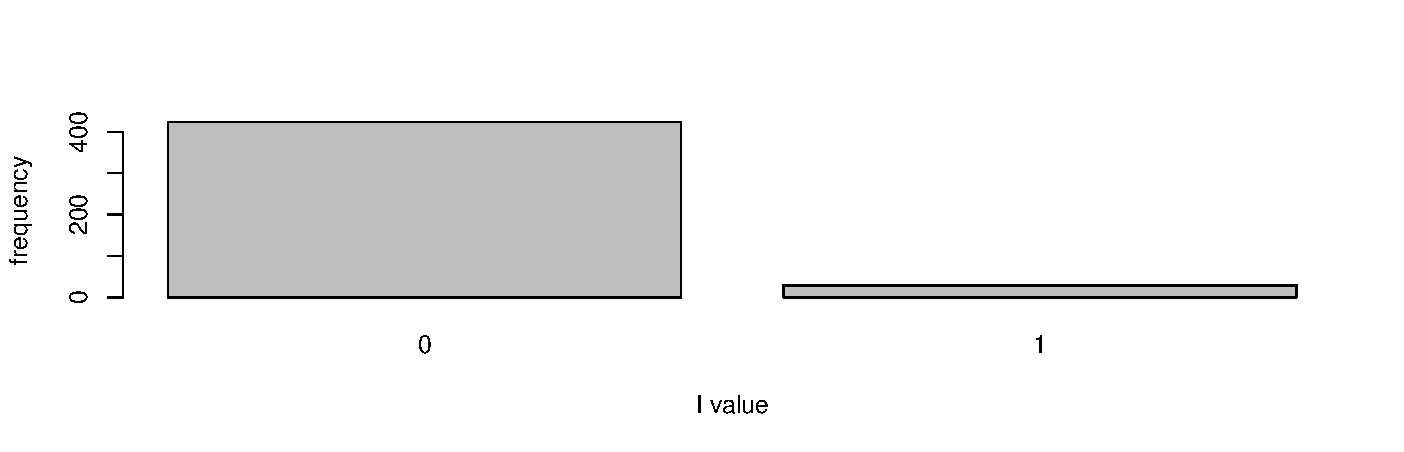
\includegraphics[width=5in]{I}
\end{figure}
\vspace{-0.5cm}

\subquestionwithpoints{2} Above is the post-burned and thinned samples from the Gibbs sampler's conditional distribution  $\cprob{I_1}{\rho, I_2, \ldots, I_n, \theta_M, \theta_F, \sigsq_M, \sigsq_F, X_1, X_2, \ldots, X_n}$. Estimate the value of $\doublehat{I}_{1, \text{MMSE}}$ to two digits. \spc{0}

\subquestionwithpoints{1} Estimate the probability that the first subject is a male. \spc{0}

\subquestionwithpoints{4} Explain a step-by-step method for drawing $X_*$, a new observation from the random variable model that produced the $\Xoneton$ data observations. Use the notation found in Table~\ref{tab:eqs} if applicable. \spc{5}

\eenum

\problem Human birth weight is known to be normally distributed. 

\begin{figure}[h]
\centering
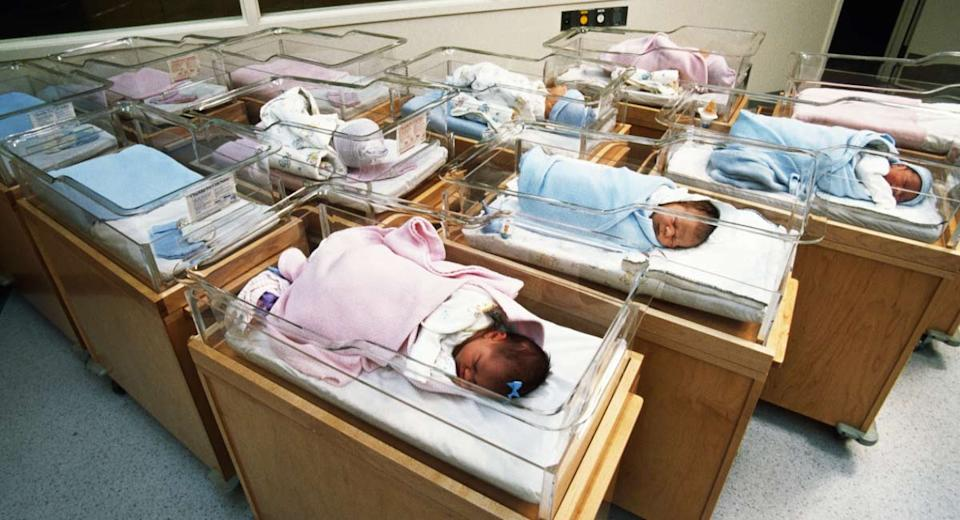
\includegraphics[width=2.5in]{babies.jpg}
\end{figure}


\noindent We measure $\braces{8.28, 7.65, 8.88, 7.80, 7.58, 6.96, 7.44, 7.34, 6.89, 6.97}$, a sample of $n=10$ birth weights measured in pounds. Its associated sample statistics are: $\xbar = 7.58$ and $s^2 = 0.39$. We cannot assume we know the true mean nor the true variance of the random variable that produced this data set. Assume Jeffrey's prior going forward.


\benum

\subquestionwithpoints{2} Find $\thetahathatmmae$ to the nearest two digits. \spc{2}
\subquestionwithpoints{3} Find $\sigsqshathatmmse$ to the nearest two digits. \spc{2.5}

\subquestionwithpoints{4} Plot the bivariate density of $\cprob{\theta,\sigsq}{X}$ as best as you can. \spc{7}

\subquestionwithpoints{4} Compute the Bayesian $p$-val for the theory that this sample's mean is underweight i.e. $H_a: \theta < 7.72$lb. \spc{3}

\subquestionwithpoints{4} Find an expression for the probability the next child in this sample will be underweight. \spc{3}


\eenum


\problem Below are some pure computation problems based on theory from this class. Solve for them using precise mathematical notation (no approximations with decimals). Simplify if possible.


\benum

\subquestionwithpoints{4} $\displaystyle \int_0^\infty x^{-17} e^{-\pi / x}dx$ \spc{2}

%\subquestionwithpoints{4} $\int_\reals e^{\pi x}e^{- x^2}dx$ \spc{2}

\subquestionwithpoints{3} $B(4,8)$ \spc{1.5}

\subquestionwithpoints{5} $\displaystyle \sum_{x=0}^n \frac{ \Gammaf{x + \alpha} \Gammaf{n - x + \beta}}{ x! (n-x)! }$ where $n \in \naturals$ and $\alpha > 0, \beta > 0$ \spc{4}


\subquestionwithpoints{5} $\displaystyle \int_\reals \tothepow{(x - \pi)^2 + 2}{-n/2}dx$ where $n \in \naturals$ \spc{5}

\eenum

\problem This question is about ratings on youtube. Each video which is voted on is either up-voted or down-voted. A video rating is the total number of thumbs up ratings over the total number of ratings. For example if a movie gets 5080 thumbs up and 960 thumbs down ratings, then it has a 5080/(5080 + 960) = 84.1\% approval rating.  

But there is a question: how should we order videos by \emph{true} approval rating $\theta \in (0,1)$? For example, here is a table of four videos we wish to order:

\begin{table}[htp]
\centering
\begin{tabular}{ccccc}
Video Name & \# Up votes & \# Down votes & $n$ & Approval Rating \\ \hline
A & 0 & 1 & 1 & 0.0\% \\
B & 4 & 0 & 4 & 100.0\% \\
C & 25 & 2 & 27 & 92.6\% \\
D & 5080 & 960 & 6040 & 84.1\% \\
\end{tabular}
\caption{Table of videos with their youtube ratings.}
\label{tab:ratings}
\end{table}

%xs = c(rbeta(2e4, 3, 1), rbeta(1e4,750, 250))
%%hist(xs, br = 100)
%fw <- fitdist(xs, "beta")
%plot(fw)
%fw



\benum

\subquestionwithpoints{1} Order the movies in Table~\ref{tab:ratings} by name from best to worst using the MLE estimate of its true approval rating. Your answer must be in the format \qu{$A > B > C > D$} where $A$ is the highest-rated and $D$ is the lowest-rated. \spc{1} %M1

\subquestionwithpoints{3} Why is what you did in (a) a poor way to order the four movies?\spc{2} %M1

\subquestionwithpoints{1} We are now going to use some previous data to create a prior for the true approval rating. What is this kind of procedure is called (two words)?\spc{0.3} %M2

Below is a histogram of the approval ratings of $n_0 = 30,000$ videos of which there are more than 200 votes each. The curve displayed atop the histogram is the best fit beta density. I used \texttt{R}'s  \texttt{fitdistrplus} package which creates a fit via the MLE's of $\alpha$ and $\beta$. I include estimates in output from \texttt{R} below the plot. 

  \begin{multicols}{2}

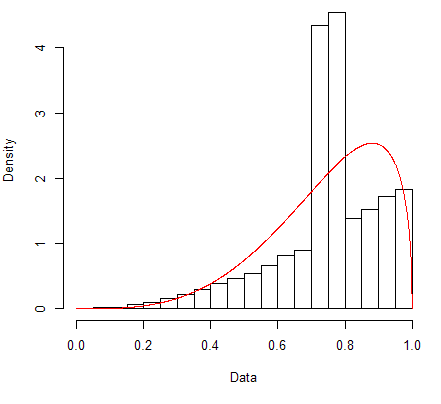
\includegraphics[width=3in]{fitdist.png}



 \begin{minipage}{0.4\linewidth}
\vspace{2cm}
\begin{verbatim}
Parameters:
       estimate Std. Error
shape1 4.283762 0.03567291
shape2 1.442157 0.01073980
\end{verbatim}
    \end{minipage}
  \end{multicols}




\subquestionwithpoints{3} Besides the fact that the curve does not fit the empirical distribution (given by the histogram), what is wrong with the estimates of $\alpha$ and $\beta$ given above? Hint: think about pseudocounts. \spc{5} %M1

\subquestionwithpoints{3} Given that a movie has $n$ total votes and $x$ of those are thumbs up, what is the posterior distribution of the true approval rating $\theta$ given the data coupled with the prior constructed above in the illustration before question (d)?\spc{1} %M1

\subquestionwithpoints{4} Order the movies in Table~\ref{tab:ratings} from best to worst using the Bayesian estimate which minimizes mean squared error. Your answer must be in the format \qu{$A > B > C > D$} where $A$ is the highest-rated and $D$ is the lowest-rated. Compute explicitly. No credit unless work is shown. \spc{3} 
\eenum

\problem Continuing the question from before, there is reason to believe that the average approval rating is trending over time. To test this, we sample the same number $n$ samples every day for $t \in \braces{1, \ldots, T}$ days and assume that $X_t \inddist \binomial{n}{\theta_t}$ where $\theta_t := \beta_0 + \beta_1 t$.

\beqn
\text{The likelihood is:}~\cprob{X_1, \ldots, X_T}{n, T, \beta_0, \beta_1} = \prod_{t=1}^T \binom{n}{x_t} \tothepow{\beta_0 + \beta_1 t}{x_t} \tothepow{1 - \beta_0 - \beta_1 t}{n - x_t}.
\eeqn

\noindent We'll assume Laplace priors for $\beta_0$ and $\beta_1$ i.e. $\prob{\beta_0, \beta_1} \propto 1$ and that $n$ is known.



\benum

\subquestionwithpoints{3} Find $k(\beta_0\,|\, \beta_1, X_1, \ldots, X_T, n, T)$. \spc{2}

\subquestionwithpoints{3} Find $k(\beta_1\,|\, \beta_0, X_1, \ldots, X_T, n, T)$. \spc{2}

\subquestionwithpoints{2} If you were to create a Gibbs sampler using both $k(\beta_0\,|\, \beta_1, X_1, \ldots, X_T, n, T)$ and $k(\beta_1\,|\, \beta_0, X_1, \ldots, X_T, n, T)$, what is the name of one algorithm that could be used when sampling $\beta_0$? \spc{0.5}

\eenum



\begin{table}[htp]
\centering
\small
\begin{tabular}{l | llll}
Distribution                  & Quantile  & PMF / PDF  &CDF       & Sampling  \\ 
of r.v. &  Function & function         & function &  Function \\ \hline
beta & \texttt{qbeta}($p$, $\alpha$, $\beta$)             
& \texttt{d-}($x$, $\alpha$, $\beta$)
& \texttt{p-}($x$, $\alpha$, $\beta$) 
& \texttt{r-}($\alpha$, $\beta$) \\
betabinomial & \texttt{qbetabinom}($p$, $n$, $\alpha$, $\beta$)              
& \texttt{d-}($x$, $n$, $\alpha$, $\beta$)
& \texttt{p-}($x$, $n$, $\alpha$, $\beta$) 
& \texttt{r-}($n$, $\alpha$, $\beta$) \\

betanegativebinomial & \texttt{qbeta\_nbinom}($p$, $r$, $\alpha$, $\beta$) 
& \texttt{d-}($x$, $r$, $\alpha$, $\beta$)
& \texttt{p-}($x$, $r$, $\alpha$, $\beta$) 
& \texttt{r-}($r$, $\alpha$, $\beta$) \\

binomial & \texttt{qbinom}($p$, $n$, $\theta$) 
& \texttt{d-}($x$, $n$, $\theta$)
& \texttt{p-}($x$, $n$, $\theta$) 
& \texttt{r-}($n$, $\theta$) \\

exponential & \texttt{qexp}($p$, $\theta$) 
& \texttt{d-}($x$, $\theta$) 
& \texttt{p-}($x$, $\theta$) 
& \texttt{r-}($\theta$) \\

gamma & \texttt{qgamma}($p$, $\alpha$, $\beta$) 
& \texttt{d-}($x$, $\alpha$, $\beta$)
& \texttt{p-}($x$, $\alpha$, $\beta$) 
& \texttt{r-}($\alpha$, $\beta$) \\

geometric & \texttt{qgeom}($p$, $\theta$) 
& \texttt{d-}($x$, $\theta$)
& \texttt{p-}($x$, $\theta$) 
& \texttt{r-}($\theta$) \\

inversegamma & \texttt{qinvgamma}($p$, $\alpha$, $\beta$) 
& \texttt{d-}($x$, $\alpha$, $\beta$)
& \texttt{p-}($x$, $\alpha$, $\beta$) 
& \texttt{r-}($\alpha$, $\beta$) \\

negative-binomial & \texttt{qnbinom}($p$, $r$, $\theta$) 
& \texttt{d-}($x$, $r$, $\theta$) 
& \texttt{p-}($x$, $r$, $\theta$) 
& \texttt{r-}($r$, $\theta$) \\

normal (univariate) & \texttt{qnorm}($p$, $\theta$, $\sigma$) 
& \texttt{d-}($x$, $\theta$, $\sigma$)
& \texttt{p-}($x$, $\theta$, $\sigma$) 
& \texttt{r-}($\theta$, $\sigma$) \\

%normal (multivariate) & 
%& \multicolumn{2}{l}{\texttt{dmvnorm}($\x$, $\muvec$, $\bSigma$)} 
%& \texttt{r-}($\muvec$, $\bSigma$) \\

poisson & \texttt{qpois}($p$, $\theta$) 
& \texttt{d-}($x$, $\theta$)
& \texttt{p-}($x$, $\theta$) 
& \texttt{r-}($\theta$) \\

T (standard) & \texttt{qt}($p$, $\nu$) 
& \texttt{d-}($x$, $\nu$) 
& \texttt{p-}($x$, $\nu$)
& \texttt{r-}($\nu$) \\

T (scaled) & \texttt{qt.scaled}($p$, $\nu$, $\mu$, $\sigma$) 
& \texttt{d-}($x$, $\nu$, $\mu$, $\sigma$)
& \texttt{p-}($x$, $\nu$, $\mu$, $\sigma$) 
& \texttt{r-}($\nu$, $\mu$, $\sigma$) \\

uniform & \texttt{qunif}($p$, $a$, $b$) 
& \texttt{d-}($x$, $a$, $b$)
& \texttt{p-}($x$, $a$, $b$) 
& \texttt{r-}($a$, $b$) \\


\end{tabular}
\caption{Functions from $\texttt{R}$ (in alphabetical order) that can be used on this exam with their arguments. The hyphen in colums 3, 4 and 5 is shorthand notation for the full text of the r.v. which can be found in column 2.
}
\label{tab:eqs}
\end{table}

\end{document}
%%%%%%%%%%%%%%%%%%%%%%%
%%%%%%%%%%%%%%%%%%%%%%%
%%%%%%%%%%%%%%%%%%%%%%%
%%%%%%%%%%%%%%%%%%%%%%%
%%%%%%%%%%%%%%%%%%%%%%%
%%%%%%%%%%%%%%%%%%%%%%%

\problem Measuring the speed of light using a laser is known to be unbiased i.e. the mean is $\theta = 299792458$ m/s.

\begin{figure}[h]
\centering
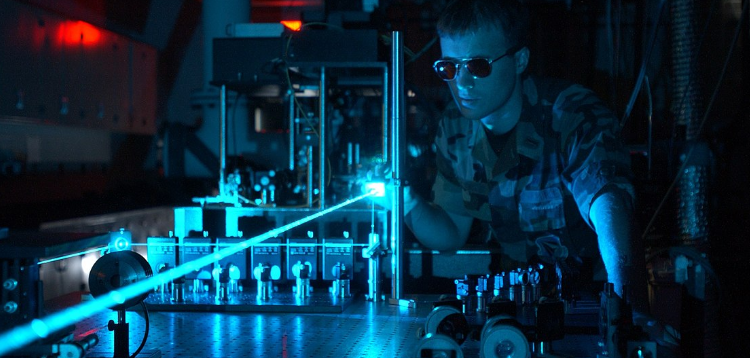
\includegraphics[width=3in]{laser.png}
\end{figure}

\noindent However, there is variance $\sigsq$ which we seek to understand. We do 3 experiments and find measurements of the speed of light to be $x_1 = 303884490$, $x_2 = 296562208$ and $x_3 = 306150981$. Assume these measurements are $\iid \normnot{\theta}{\sigsq}$.

\benum

\subquestionwithpoints{4} Find $\sigsqshathatmle$. \spc{2}

\subquestionwithpoints{4} What is the Jeffrey's prior for $\sigsq~|~\theta$? \spc{0}

\subquestionwithpoints{4} Using Jeffrey's prior for $\sigsq~|~\theta$, find the posterior distribution $\cprob{\sigsq}{X, \theta}$. \spc{1}

\subquestionwithpoints{6} Write the PDF of $\cprob{\sigsq}{X, \theta}$ explicitly. \spc{3}

\subquestionwithpoints{6} Compute $\sigsqshathatmap$. \spc{3}

\subquestionwithpoints{6} Express the $CR_{\sigsq, 90\%}$ using Table 1. \spc{2}

\subquestionwithpoints{6} Express the probability the next experiment will have a measurement different from the truth by more than 1,000 m/s using Table 1. \spc{3}

\eenum



\problem Ladislaus Josephovich Bortkiewicz was a Polish economist and statistician who published a book in 1898 about the Poisson distribution. A famous dataset in this book is the \qu{Prussian horse-kicking data} famous. 


\begin{figure}[h]
\centering
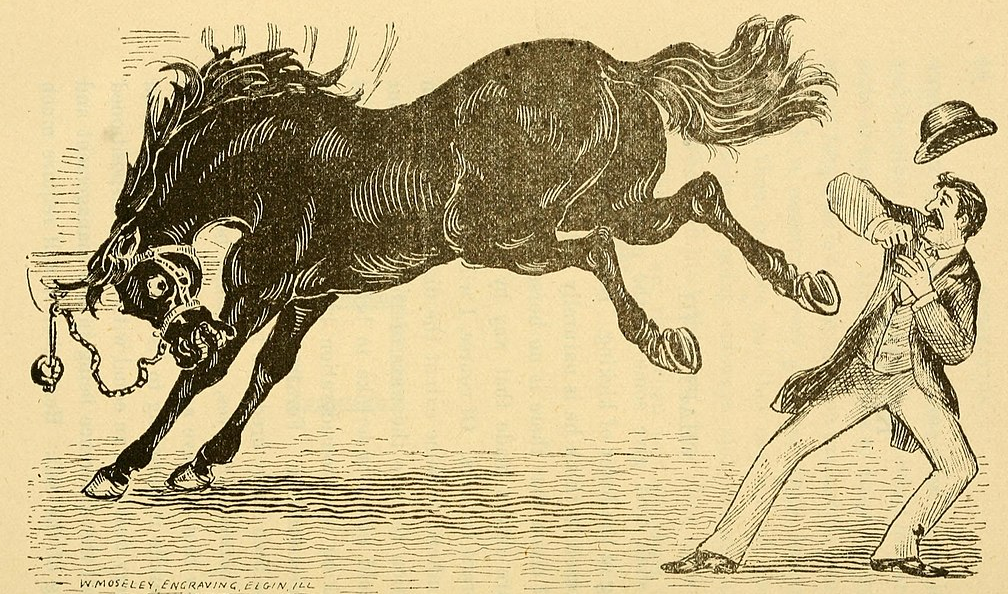
\includegraphics[width=3in]{horse.png}
\end{figure}

\noindent The data gave the number of soldiers killed by being kicked by a horse each year in each of 16 different cavalry corps over a 20-year period. Bortkiewicz showed that those numbers followed a Poisson distribution and hence we can assume the following data for the general corps is $\iid \poisson{\theta}$.

\begin{table}[h]
\footnotesize
\begin{tabular}{l|cccccccccccccccccccc}
Year (18--)	& 75 & 76 & 77 & 78 & 79 & 80 & 81 & 82 & 83 & 84 & 85 & 86 & 87 & 88 & 89 & 90 & 91 & 92 & 93 & 94 \\ \hline
\# kicks &	0	& 2	& 2	& 1	& 0	& 0	& 1	& 1	& 0	& 3	& 0	& 2	& 1	& 0	& 0	& 1	& 0	& 1	& 0	& 1 \\
\end{tabular}
\end{table}

\benum

\subquestionwithpoints{4} In this example, what is the interpretation of the parameter $\theta$? Answer using English sentence(s). \spc{2}

\subquestionwithpoints{4} What is Haldane's prior for $\theta$? \spc{0}

\subquestionwithpoints{2} Is Haldane's prior for $\theta$ proper? Yes / no. \spc{-0.5}

\subquestionwithpoints{4} Using Haldane's prior for $\theta$, find the posterior distribution $\cprob{\theta}{X}$. \spc{1}


\subquestionwithpoints{2} Is $\cprob{\theta}{X}$ proper? Yes / no. \spc{-0.5}

\subquestionwithpoints{4} Compute $\thetahathatmmse$. \spc{3}

\subquestionwithpoints{5} Express the $CR_{\theta, 95\%}$ below using Table 1. \spc{2}

\subquestionwithpoints{7} Express the Bayesian p-value when testing the hypothesis that $\theta > 1$ using Table 1. \spc{2}

\subquestionwithpoints{7} Express the probability the number of kicks in 1895 is three or more using Table 1. \spc{1}

\eenum


\pagebreak


\problem Every worker at the chocolate factory must wrap the chocolate desserts. 

\begin{figure}[h]
\centering
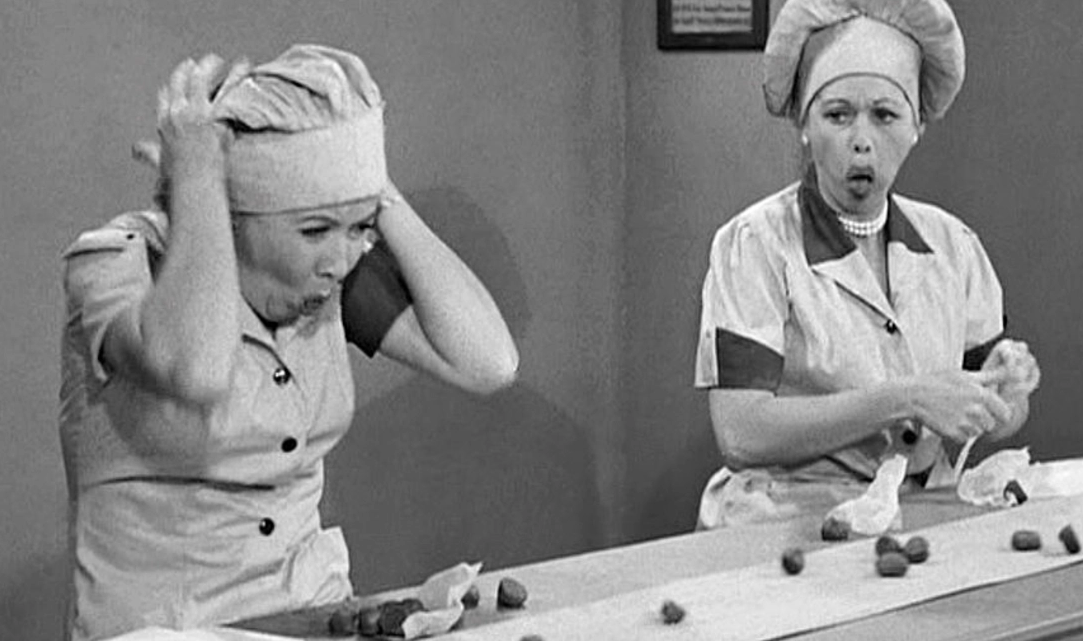
\includegraphics[width=3in]{chocolate.png}
\end{figure}

\noindent Each dessert takes a variable amount of time to wrap. We can assume since wrapping has many factors summed, an $\iid \normnot{\theta}{\sigsq}$ is a good model where $\sigsq$ is known to be 0.01 seconds-squared. However, every worker has a different $\theta$. 

A new worker is hired and we naturally want to see how fast this worker wraps on average. For the first three wrappings, the worker does it in 0.23 seconds, 0.21 seconds and 0.24 seconds for an average of $\xbar = 0.2267$ seconds. This is remarkably fast relative to other workers so it is unrealistic to assume this is a good estimate of this new worker's true $\theta$. Here are other worker's lifetime averages:

\begin{figure}[h]
\centering
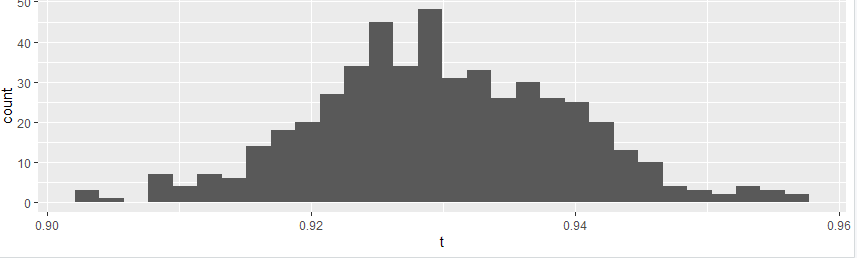
\includegraphics[width=5in]{hist.png}
\end{figure}

\noindent Fitting a normal distribution to this data and using maximum likelihood, we find the average worker lifetime wrapping time average is 0.930 seconds with a variance of 0.0000927 seconds-squared. We would like to use the empirical Bayes estimation to draw inference for the new worker's $\theta$.


\benum


\subquestionwithpoints{5} If we use the normal fit of other workers' lifetime averages to create a prior, this prior will be equivalent to how many pseudoobservations $n_0$? \spc{4}

\subquestionwithpoints{2} Is this prior uninformative? Yes / no. \spc{-0.5}

\subquestionwithpoints{5} Compute $\thetahathatmmae$ under this prior. \spc{5}

\subquestionwithpoints{5} Calculate the shrinkage $\rho$ for this $\thetahathatmmae$ estimate under this prior. \spc{4}

\subquestionwithpoints{8} Express the probability that this new worker is better than average under this prior using Table 1. \spc{3}
\eenum


\pagebreak
\begin{table}[htp]
\centering
\small
\begin{tabular}{l | llll}
Distribution                  & Quantile  & PMF / PDF  &CDF       & Sampling  \\ 
of r.v. &  Function & function         & function &  Function \\ \hline
beta & \texttt{qbeta}($p$, $\alpha$, $\beta$)             
& \texttt{d-}($x$, $\alpha$, $\beta$)
& \texttt{p-}($x$, $\alpha$, $\beta$) 
& \texttt{r-}($\alpha$, $\beta$) \\
betabinomial & \texttt{qbetabinom}($p$, $n$, $\alpha$, $\beta$)              
& \texttt{d-}($x$, $n$, $\alpha$, $\beta$)
& \texttt{p-}($x$, $n$, $\alpha$, $\beta$) 
& \texttt{r-}($n$, $\alpha$, $\beta$) \\

betanegativebinomial & \texttt{qbeta\_nbinom}($p$, $r$, $\alpha$, $\beta$) 
& \texttt{d-}($x$, $r$, $\alpha$, $\beta$)
& \texttt{p-}($x$, $r$, $\alpha$, $\beta$) 
& \texttt{r-}($r$, $\alpha$, $\beta$) \\

binomial & \texttt{qbinom}($p$, $n$, $\theta$) 
& \texttt{d-}($x$, $n$, $\theta$)
& \texttt{p-}($x$, $n$, $\theta$) 
& \texttt{r-}($n$, $\theta$) \\

exponential & \texttt{qexp}($p$, $\theta$) 
& \texttt{d-}($x$, $\theta$) 
& \texttt{p-}($x$, $\theta$) 
& \texttt{r-}($\theta$) \\

gamma & \texttt{qgamma}($p$, $\alpha$, $\beta$) 
& \texttt{d-}($x$, $\alpha$, $\beta$)
& \texttt{p-}($x$, $\alpha$, $\beta$) 
& \texttt{r-}($\alpha$, $\beta$) \\

geometric & \texttt{qgeom}($p$, $\theta$) 
& \texttt{d-}($x$, $\theta$)
& \texttt{p-}($x$, $\theta$) 
& \texttt{r-}($\theta$) \\

inversegamma & \texttt{qinvgamma}($p$, $\alpha$, $\beta$) 
& \texttt{d-}($x$, $\alpha$, $\beta$)
& \texttt{p-}($x$, $\alpha$, $\beta$) 
& \texttt{r-}($\alpha$, $\beta$) \\

negative-binomial & \texttt{qnbinom}($p$, $r$, $\theta$) 
& \texttt{d-}($x$, $r$, $\theta$) 
& \texttt{p-}($x$, $r$, $\theta$) 
& \texttt{r-}($r$, $\theta$) \\

normal (univariate) & \texttt{qnorm}($p$, $\theta$, $\sigma$) 
& \texttt{d-}($x$, $\theta$, $\sigma$)
& \texttt{p-}($x$, $\theta$, $\sigma$) 
& \texttt{r-}($\theta$, $\sigma$) \\

%normal (multivariate) & 
%& \multicolumn{2}{l}{\texttt{dmvnorm}($\x$, $\muvec$, $\bSigma$)} 
%& \texttt{r-}($\muvec$, $\bSigma$) \\

poisson & \texttt{qpois}($p$, $\theta$) 
& \texttt{d-}($x$, $\theta$)
& \texttt{p-}($x$, $\theta$) 
& \texttt{r-}($\theta$) \\

T (standard) & \texttt{qt}($p$, $\nu$) 
& \texttt{d-}($x$, $\nu$) 
& \texttt{p-}($x$, $\nu$)
& \texttt{r-}($\nu$) \\

T (scaled) & \texttt{qt.scaled}($p$, $\nu$, $\mu$, $\sigma$) 
& \texttt{d-}($x$, $\nu$, $\mu$, $\sigma$)
& \texttt{p-}($x$, $\nu$, $\mu$, $\sigma$) 
& \texttt{r-}($\nu$, $\mu$, $\sigma$) \\

uniform & \texttt{qunif}($p$, $a$, $b$) 
& \texttt{d-}($x$, $a$, $b$)
& \texttt{p-}($x$, $a$, $b$) 
& \texttt{r-}($a$, $b$) \\


\end{tabular}
\caption{Functions from $\texttt{R}$ (in alphabetical order) that can be used on this exam with their arguments. The hyphen in colums 3, 4 and 5 is shorthand notation for the full text of the r.v. which can be found in column 2.
}
\label{tab:eqs}
\end{table}

\end{document}




\problem Measuring the speed of light using a laser is known to be unbiased i.e. the mean is $\theta = 3.0 \times 10^8$ m/s. However, there is variance $\sigsq$ which we seek to understand.

\benum

\subquestionwithpoints{4} Find $\thetahatmle$. \spc{0}

%\subquestionwithpoints{4} What is the main problem with your estimate in (a)? \spc{2}

\subquestionwithpoints{5} Compute a $CI_{\theta, 95\%}$. The applicable $z_{\alpha/2} = 2$ for this confidence interval. \spc{2}

\subquestionwithpoints{5} Does the interval in (c) fulfill the second goal of statistical inference? Yes / no and explain your answer. \spc{6}


\subquestionwithpoints{5} We will now conduct Bayesian inference. Consider the reduced parameter space $\Theta_0 = \braces{1/3, 1/2, 2/3} \subset \Theta = (0, 1)$. We believe strongly in $\theta = 0.5$ but we want to give some credence to the alternate values. Thus we establish a prior of 

\beqn
\prob{\theta} = \begin{cases}
1/3 \withprob 0.1 \\ 
1/2 \withprob 0.8 \\ 
2/3 \withprob 0.1 \\ 
\end{cases}
\eeqn

Is this the \qu{prior of indifference} for the reduced parameter space? Yes / no. If yes, explain why. If no, what would the prior of indifference be?\spc{2}


\subquestionwithpoints{7} Find $\prob{X = x}$. \spc{5}

\subquestionwithpoints{7} Find $\thetahatmap$. Show all work. \spc{7}

\subquestionwithpoints{4} We will now consider the entire parameter space for the binomial model i.e. $\Theta = (0, 1)$. We will use the prior $\theta \sim \betanot{0}{0}$. We will see later in class that this is called \qu{Haldane's prior of ignorance}. Is this prior a legal rv? Circle one: yes / no.\spc{-0.5}

\subquestionwithpoints{4} Regardless of the answer to your previous question, how many pseudofailures is represented by this prior?\spc{0.5}


\subquestionwithpoints{4} We will use the prior $\theta \sim \betanot{0.1}{0.1}$. Is this prior a legal rv? Circle one: yes / no.\spc{-0.5}

\subquestionwithpoints{4} Assuming the prior in (i), $\cprob{\theta}{X = x} =$ \spc{0}

\subquestionwithpoints{10} Draw $\cprob{\theta}{X = x}$ from (j) to the best of your ability. Label all axes and critical points. \spc{6}

\subquestionwithpoints{4} Does $\thetahatmap$ exist? Circle one: yes / no. \spc{-0.5}

\subquestionwithpoints{4} Compute $\thetahatmmse$ (4pt). Denote it in the illustration above (1pt). \spc{1}

\subquestionwithpoints{4} Express $\thetahatmmae$ but do not compute (4pt). Denote it in the illustration above (1pt). \spc{0.5}

\subquestionwithpoints{4} What is the proportion of shrinkage towards the prior expectation if you employ the posterior expectation as your point estimate? \spc{1}


\eenum

\problem Consider $\Xoneton \iid \text{Rayleigh}\parens{\theta} := \frac{x}{\theta}e^{-x^2 / (2\theta)}$ which has support $(0,\infty)$ and parameter space $\Theta = (0, \infty)$.

\benum

\subquestionwithpoints{8} Find $\loglik{\theta ; \Xoneton}$. Simplify as much as possible.\spc{5}

\subquestionwithpoints{9} Find $\thetahatmle$. \spc{6}

\eenum

\problem The following are theoretical questions.

\benum

\subquestionwithpoints{8} Compute $B(5,5)^{-1}$.\spc{3}

\subquestionwithpoints{6} Extra credit: compute $B(0.5,0.5)$. Do this on the back of this page. \spc{3}

\eenum


\end{document}
